\section{Q1:Visualization of k-means codebook's quantization result of sample training / testing images}
\label{subsec:Q1_histograms}
In \cref{fig:q1_histogram_tr} and \cref{fig:q1_histogram_te}, we visualized the quantization results of training and testing images using our k-means vocabulary, along with their corresponding image. Even with the same 100K SIFT feature descriptor as input, the vector quantization results vary significantly depending on the value of $K$.//

\begin{figure}[htbp]
	\centering
	\begin{subfigure}[t]{0.3\linewidth}
		\centering
		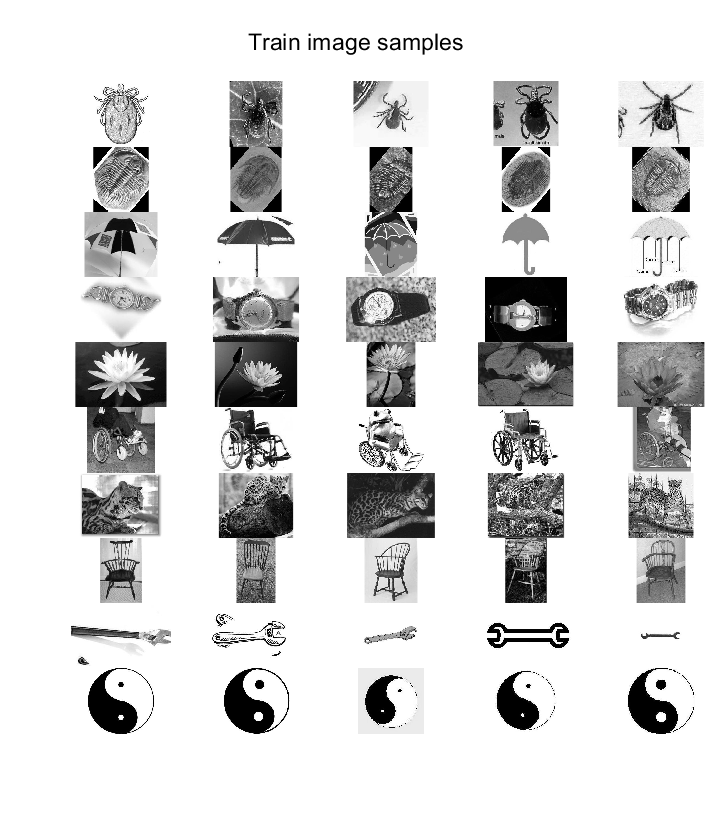
\includegraphics[height=6cm]{image/q1-appendix/train_img.png} 
		\caption{Train image samples}
	\end{subfigure}%
	\hfill
	\begin{subfigure}[t]{0.3\linewidth}
		\centering
		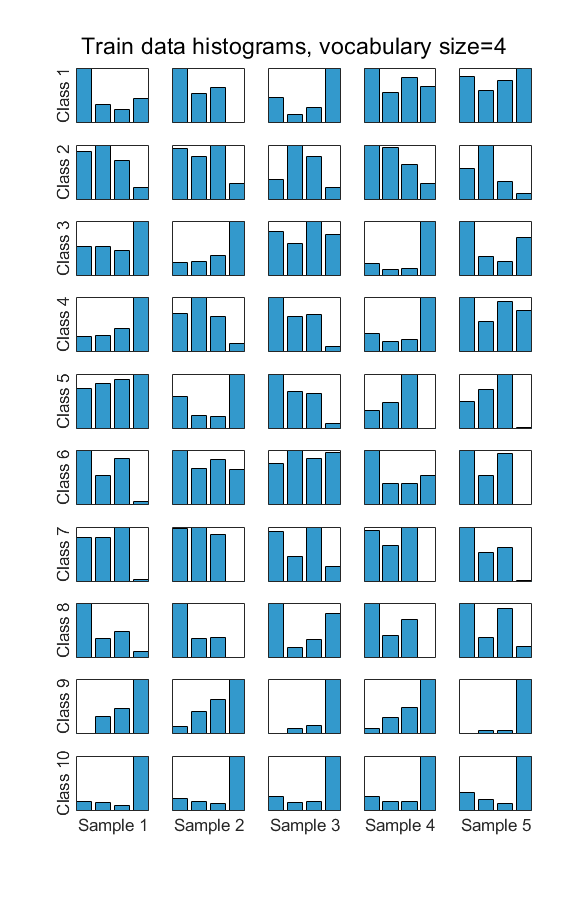
\includegraphics[height=6cm]{image/q1-appendix/train_4.png}
		\caption{Train data quantisation result, $K=4$}
	\end{subfigure}
	\hfill
	\begin{subfigure}[t]{0.3\linewidth}
		\centering
		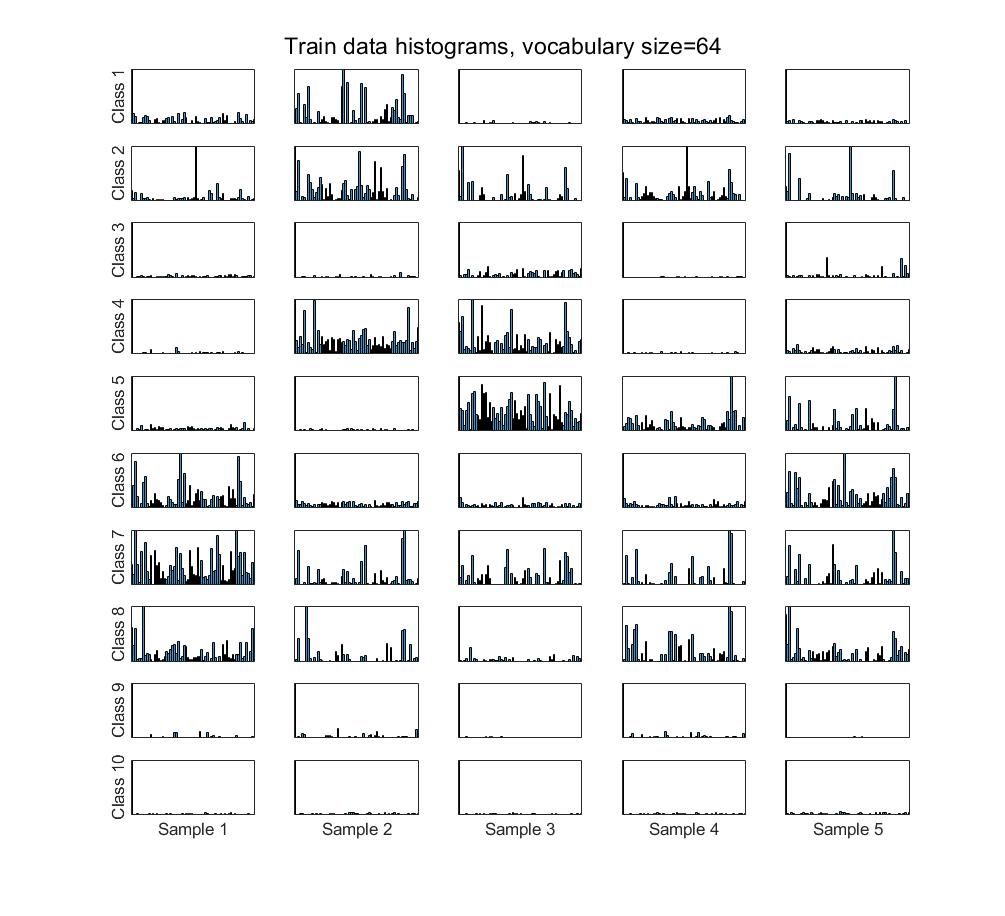
\includegraphics[height=6cm]{image/q1-appendix/train_64.png}
		\caption{Train data quantisation result, $K=64$}
	\end{subfigure}
	\caption{K-means vocabulary: Visualistaion of train data quantisation result}
	\label{fig:q1_histogram_tr}
\end{figure}

\begin{figure}[htbp]
	\centering
	\begin{subfigure}[t]{0.3\linewidth}
		\centering
		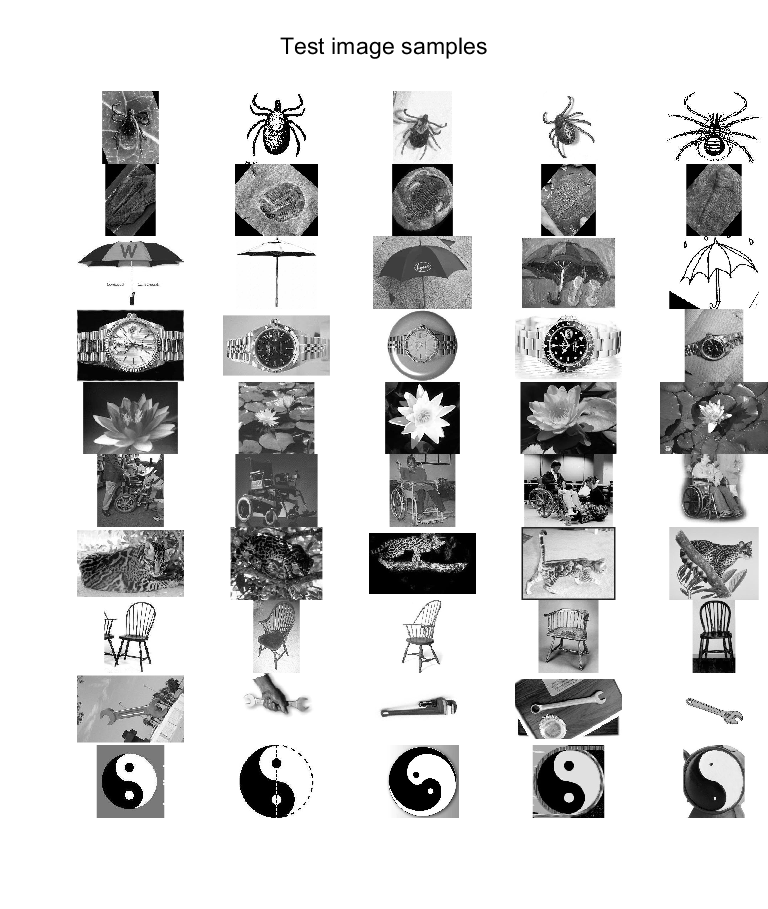
\includegraphics[height=6cm]{image/q1-appendix/test_img.png} 
		\caption{Test image samples}
	\end{subfigure}%
	\hfill
	\begin{subfigure}[t]{0.3\linewidth}
		\centering
		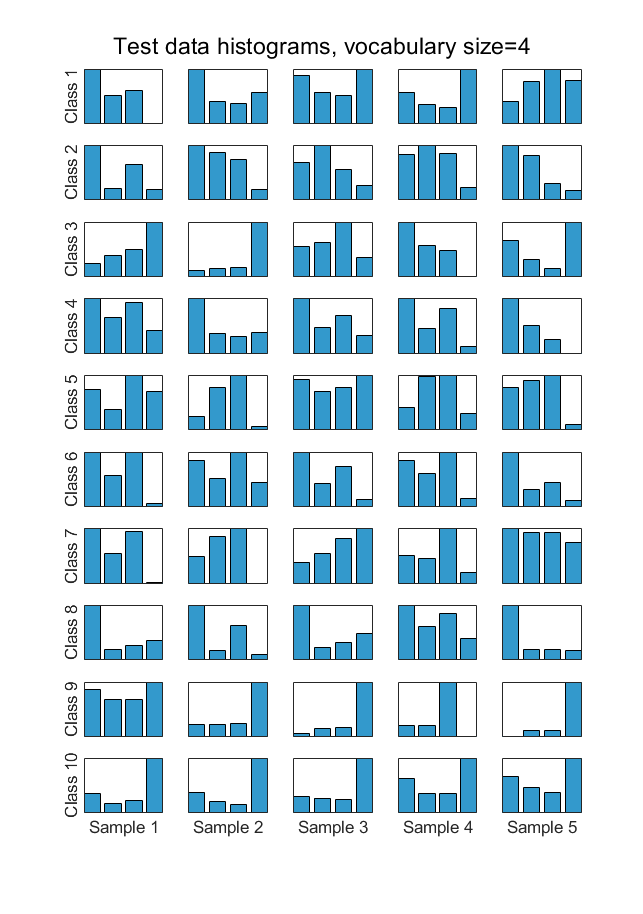
\includegraphics[height=6cm]{image/q1-appendix/test_4.png}
		\caption{Test data quantisation result, $K=4$}
	\end{subfigure}
	\hfill
	\begin{subfigure}[t]{0.3\linewidth}
		\centering
		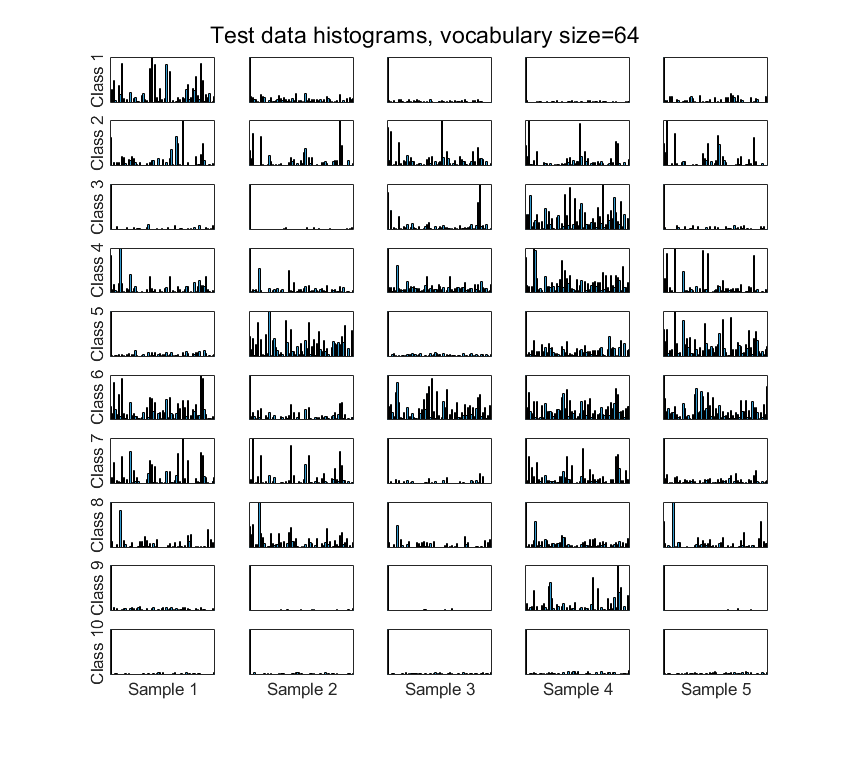
\includegraphics[height=6cm]{image/q1-appendix/test_64.png}
		\caption{Test data quantisation result, $K=64$}
	\end{subfigure}
	\caption{K-means vocabulary: Visualistaion of test data quantisation result}
	\label{fig:q1_histogram_te}
\end{figure}

\section{Q1:Cosine similarity between images in \cref{fig:q1-fig2}}
In \cref{subsec:Q1_2}, we discussed the inner-class cosine similarity and between-class cosine similarity. As shown in \cref{fig:q1_cossim}, we can observe that the similarity between images from different classes is higher than the similarity within the same class, which could lead to an underfitting issue. However, as $K$ increases, the similarity between images within the same class becomes larger than the similarity between different class images, which is good for after classification operations. Furthermore, if the vocabulary size is too large, the similarity between inner-class images also decreases because our vector quantization may capture unnecessary details for classification, potentially leading to overfitting.

\label{subsec:Q1_cossim}
\begin{figure}[htbp]
	\centering
	\begin{subfigure}[t]{0.25\linewidth}
		\centering
		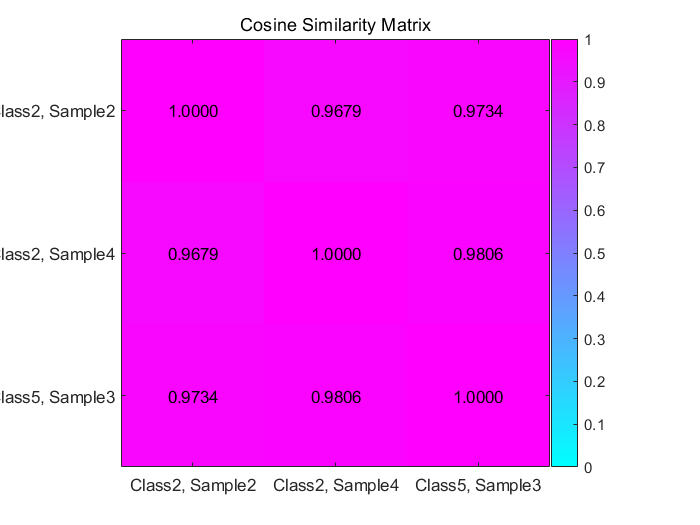
\includegraphics[width=\linewidth]{image/q1-appendix/similarity_4.png} 
		\caption{$K=4$}
	\end{subfigure}%
	\hfill
	\begin{subfigure}[t]{0.25\linewidth}
		\centering
		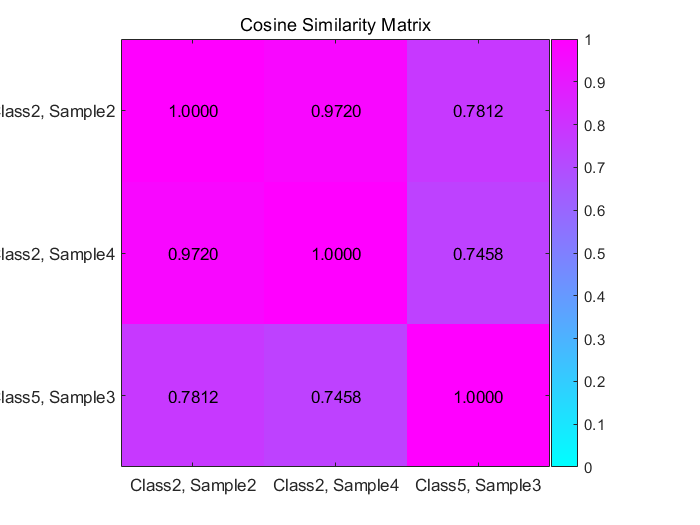
\includegraphics[width=\linewidth]{image/q1-appendix/similarity_16.png} 
		\caption{$K=16$}
	\end{subfigure}%
	\hfill
	\begin{subfigure}[t]{0.25\linewidth}
		\centering
		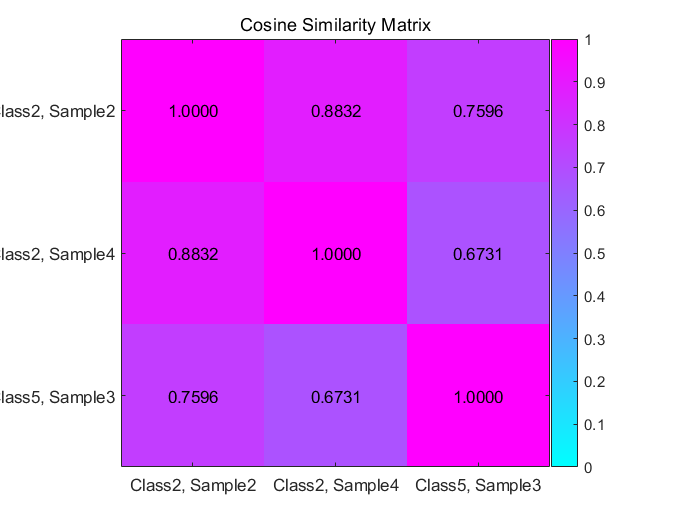
\includegraphics[width=\linewidth]{image/q1-appendix/similarity_64.png} 
		\caption{$K=64$}
	\end{subfigure}%
	\hfill
	\begin{subfigure}[t]{0.25\linewidth}
		\centering
		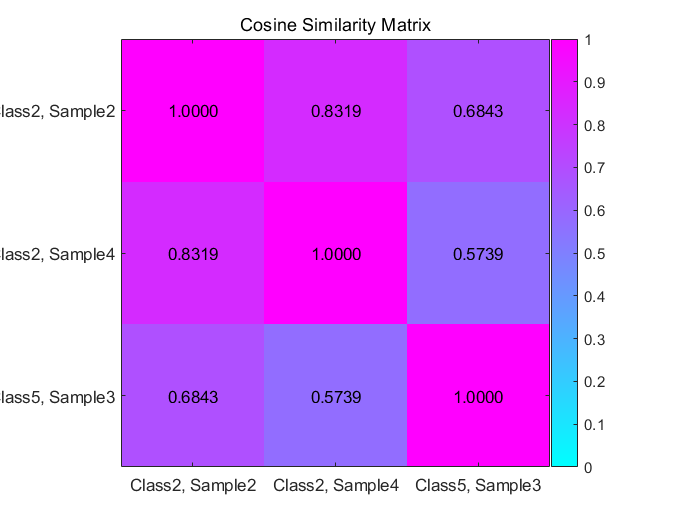
\includegraphics[width=\linewidth]{image/q1-appendix/similarity_256.png} 
		\caption{$K=256$}
	\end{subfigure}%
	\caption{Visualization of cosine similarity matrix of \cref{fig:q1-fig2} according to the different $K$}
	\label{fig:q1_cossim}
\end{figure}

\section{Q2: Test result's confusion matrix and success/failure cases}
\label{subsec:Q2-app1}
The optimal parameters determined for the random classification forest through experiments are $N=250$, $D=8$, and $\text{splitnum}=10$. With this configuration, each real-time executable weak learner—axis-aligned and two-pixel tests—each was trained 10 times. The confusion matrix results in \cref{fig:APP-q2-fig1} represent the best test accuracy among the 10 repetitive train results.\\
As a result, we can observe that the information gain of the two-pixel test is significantly higher. Referring to \cref{fig:APP-q2-fig1}, it is evident that the accuracy for all classes is generally higher in the two-pixel weak learner compared to the axis-aligned weak learner.\\
Also, you can see the example success and failure cases of random forest codebook at \cref{fig:APP-q2-case1}, \cref{fig:APP-q2-case2}.

\begin{figure}[htbp]
	\centering
	\begin{subfigure}[t]{0.4\linewidth}
		\centering
		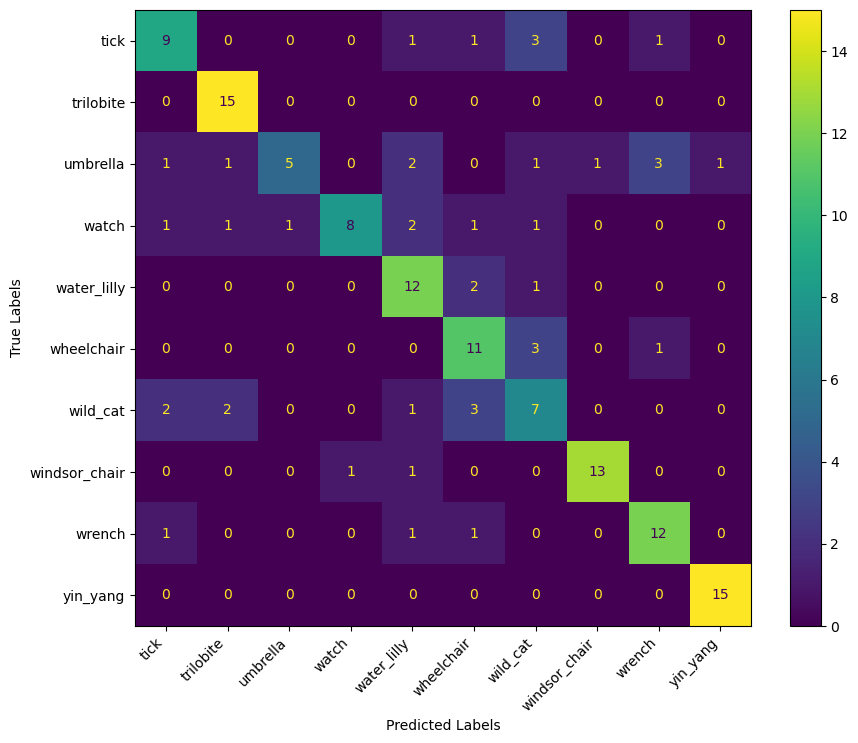
\includegraphics[width=\linewidth]{image/conf-appendix/km_axis_confusion.png}
		\caption{Axis-aligned weak learner, test accuracy=0.713}
		\label{fig:q2-appfig1}
	\end{subfigure}%
	\quad
	\begin{subfigure}[t]{0.4\linewidth}
		\centering
		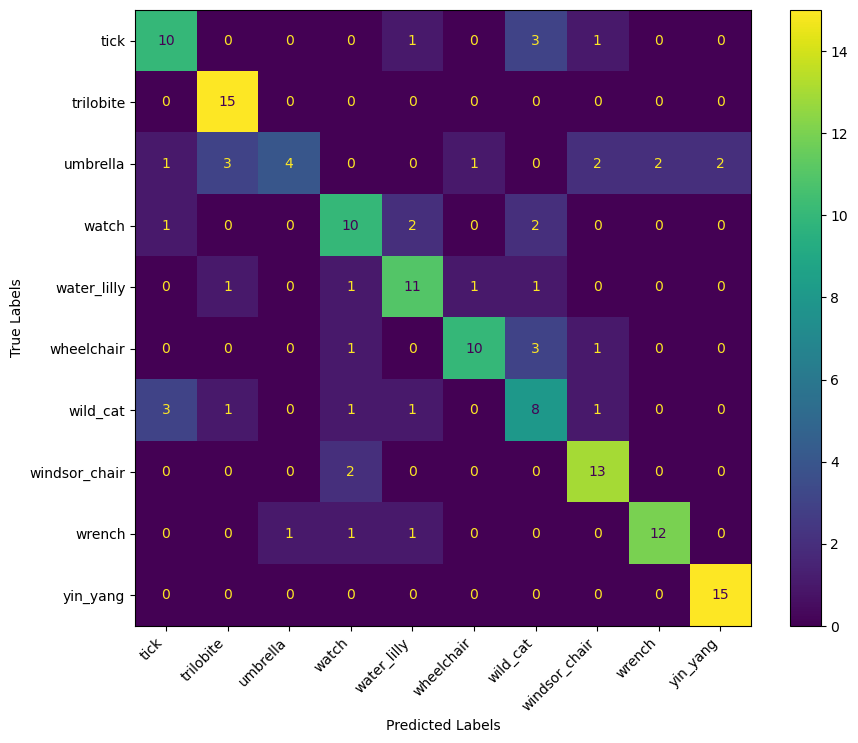
\includegraphics[width=\linewidth]{image/conf-appendix/km_twopix_confusion.png}
		\caption{Two-pixel test weak learner, test accuracy=0.720}
		\label{fig:q2-appfig2}
	\end{subfigure}
	\caption{Confusion matrix of optimal cases ($N=250$, $D=8$, and $\text{splitnum}=10$) with K-means codebook}
	\label{fig:APP-q2-fig1}
\end{figure}

\begin{figure}[htbp]
	\centering
	\begin{subfigure}{0.45\linewidth}
		\centering
		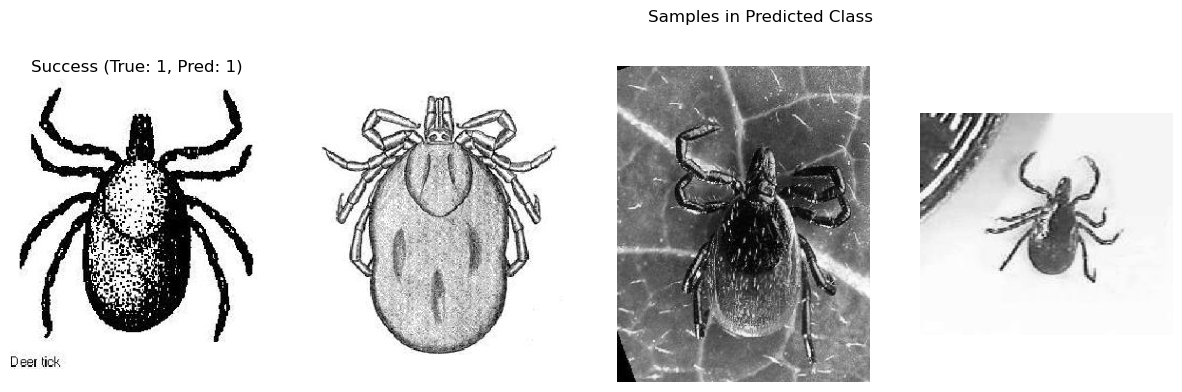
\includegraphics[width=\linewidth]{image/conf-appendix/km_axis_succ1.png}
	\end{subfigure}%
	\quad
	\begin{subfigure}{0.45\linewidth}
		\centering
		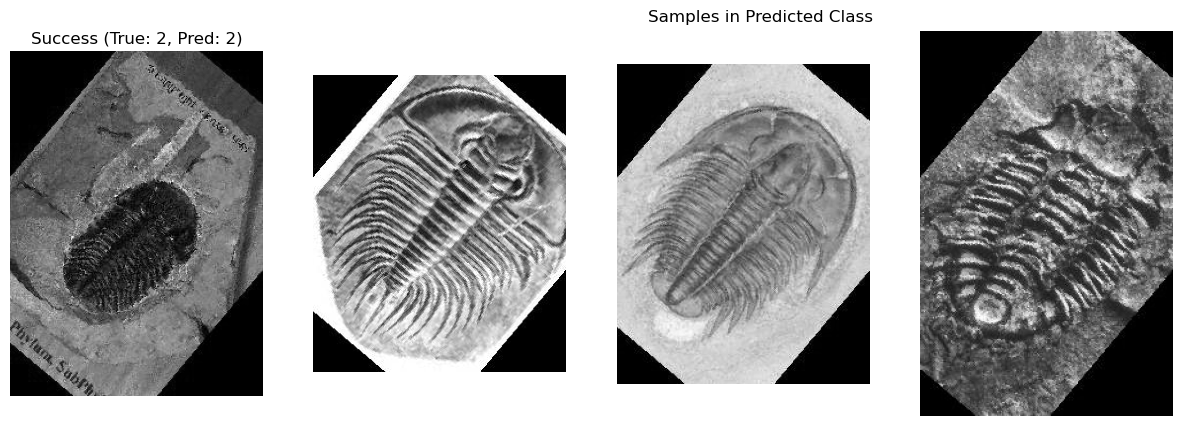
\includegraphics[width=\linewidth]{image/conf-appendix/km_axis_succ2.png}
	\end{subfigure}
	\caption{K-means codebook with axis-aligned RF classifier: Example success case}
	\label{fig:APP-q2-case1}
\end{figure}
\begin{figure}[htbp]
	\centering
	\begin{subfigure}[t]{0.45\linewidth}
		\centering
		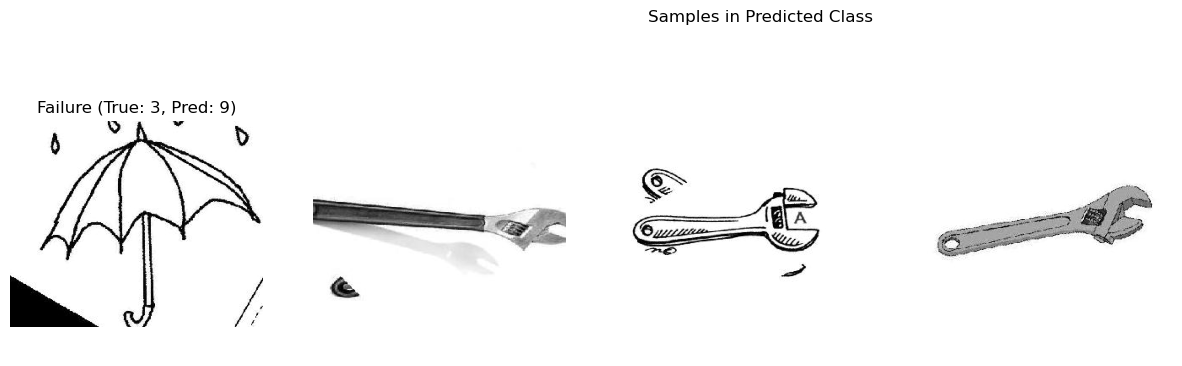
\includegraphics[width=\linewidth]{image/conf-appendix/km_axis_fail2.png}
	\end{subfigure}%
	\quad
	\begin{subfigure}[t]{0.45\linewidth}
		\centering
		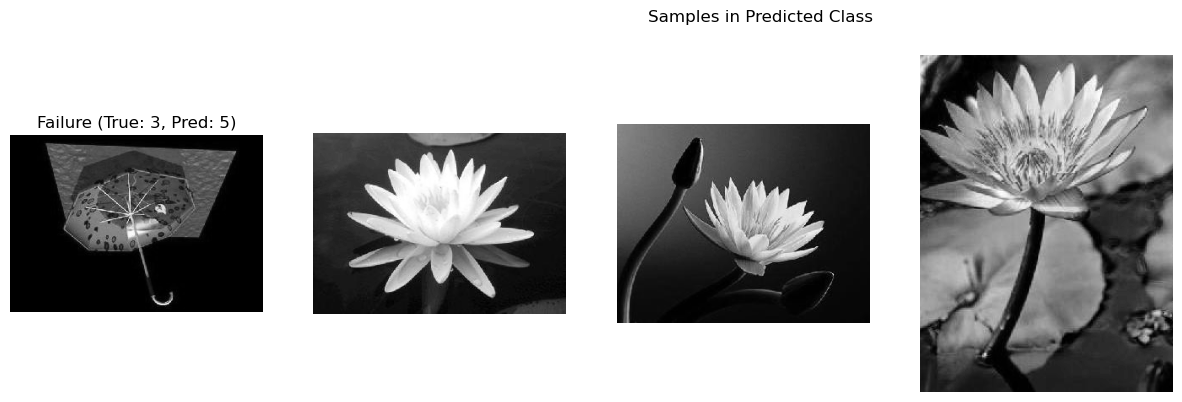
\includegraphics[width=\linewidth]{image/conf-appendix/km_axis_fail3.png}
	\end{subfigure}
	\caption{K-means codebook with axis-aligned RF classifier: Example failure case}
	\label{fig:APP-q2-case2}
\end{figure}

\section{Q2: Visualization of random forest's information gain process}
\label{subsec:Q2-app2}


\section{Q3: Optimization process of Random forest vocabulary}
Following a procedure similar to \cref{sec:intro_q2}, we determined the optimal parameters for the random forest vocabulary. The results are shown in \cref{fig:q3-app-fig1} and \cref{fig:q3-app-fig2}. Consequently, the optimal parameters determined for the random classification forest through experiments are $N=8$, $D=6$, and $\text{splitnum}=10$.

\label{subsec:Q2-app3}
\begin{figure}[htbp]
	\centering
	\begin{subfigure}[H]{0.7\linewidth}
		\centering
		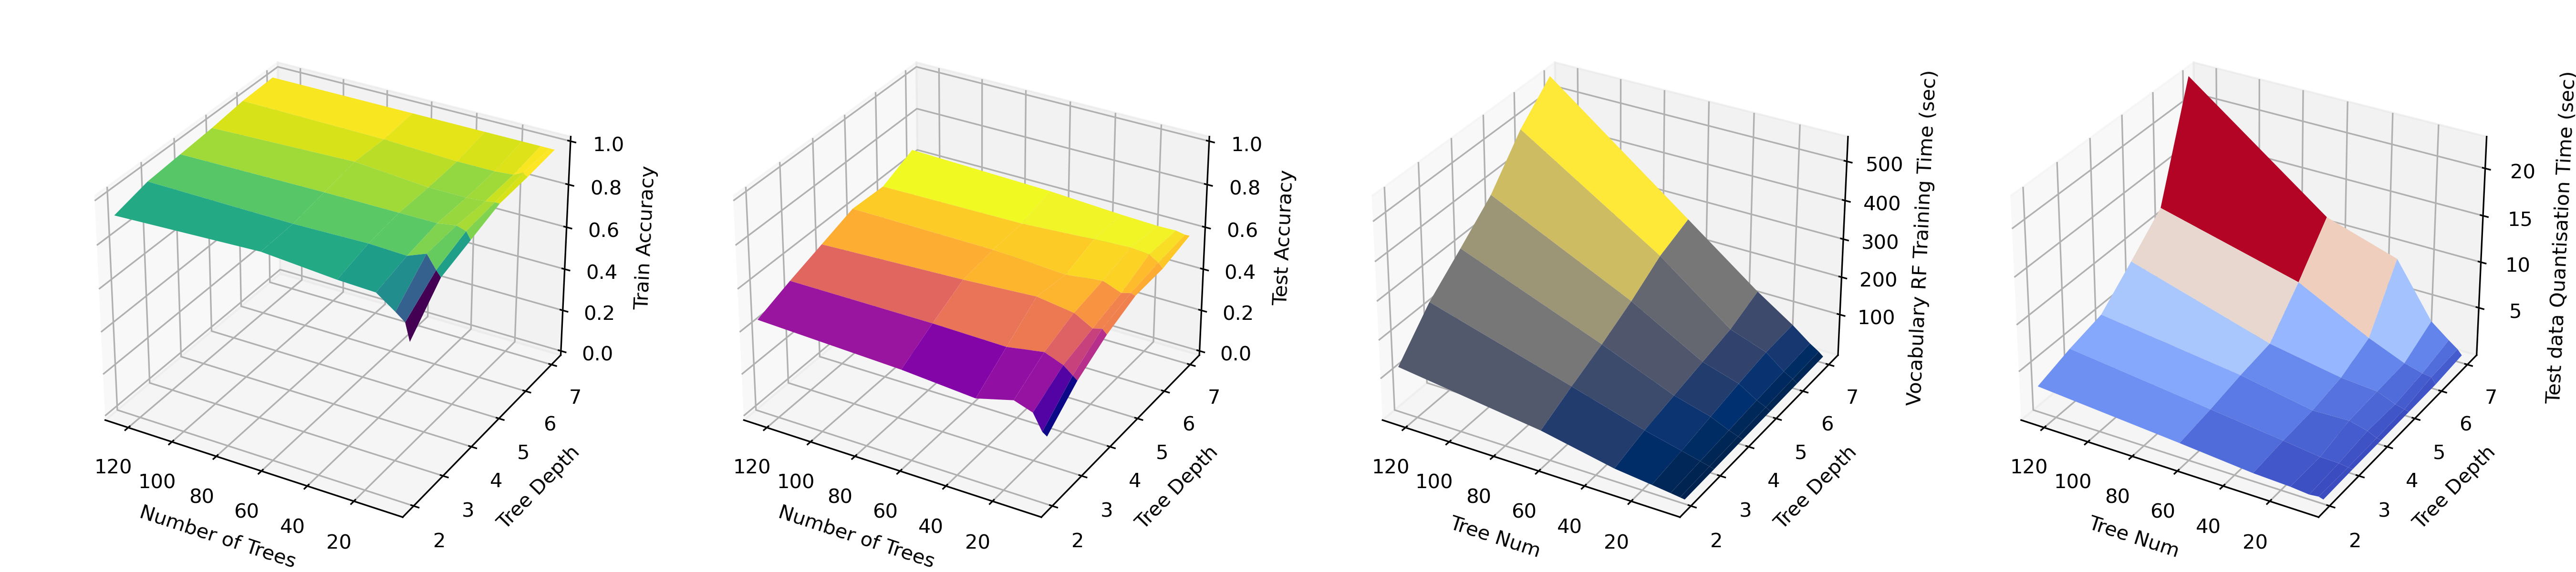
\includegraphics[width=\linewidth]{image/q3-fig1.png}
		\caption{Training\&Testing accuracy and time according to the number of tree and the depth of tree}
		\label{fig:q3-fig1}
	\end{subfigure}
	\begin{subfigure}[H]{0.7\linewidth}
		\centering
		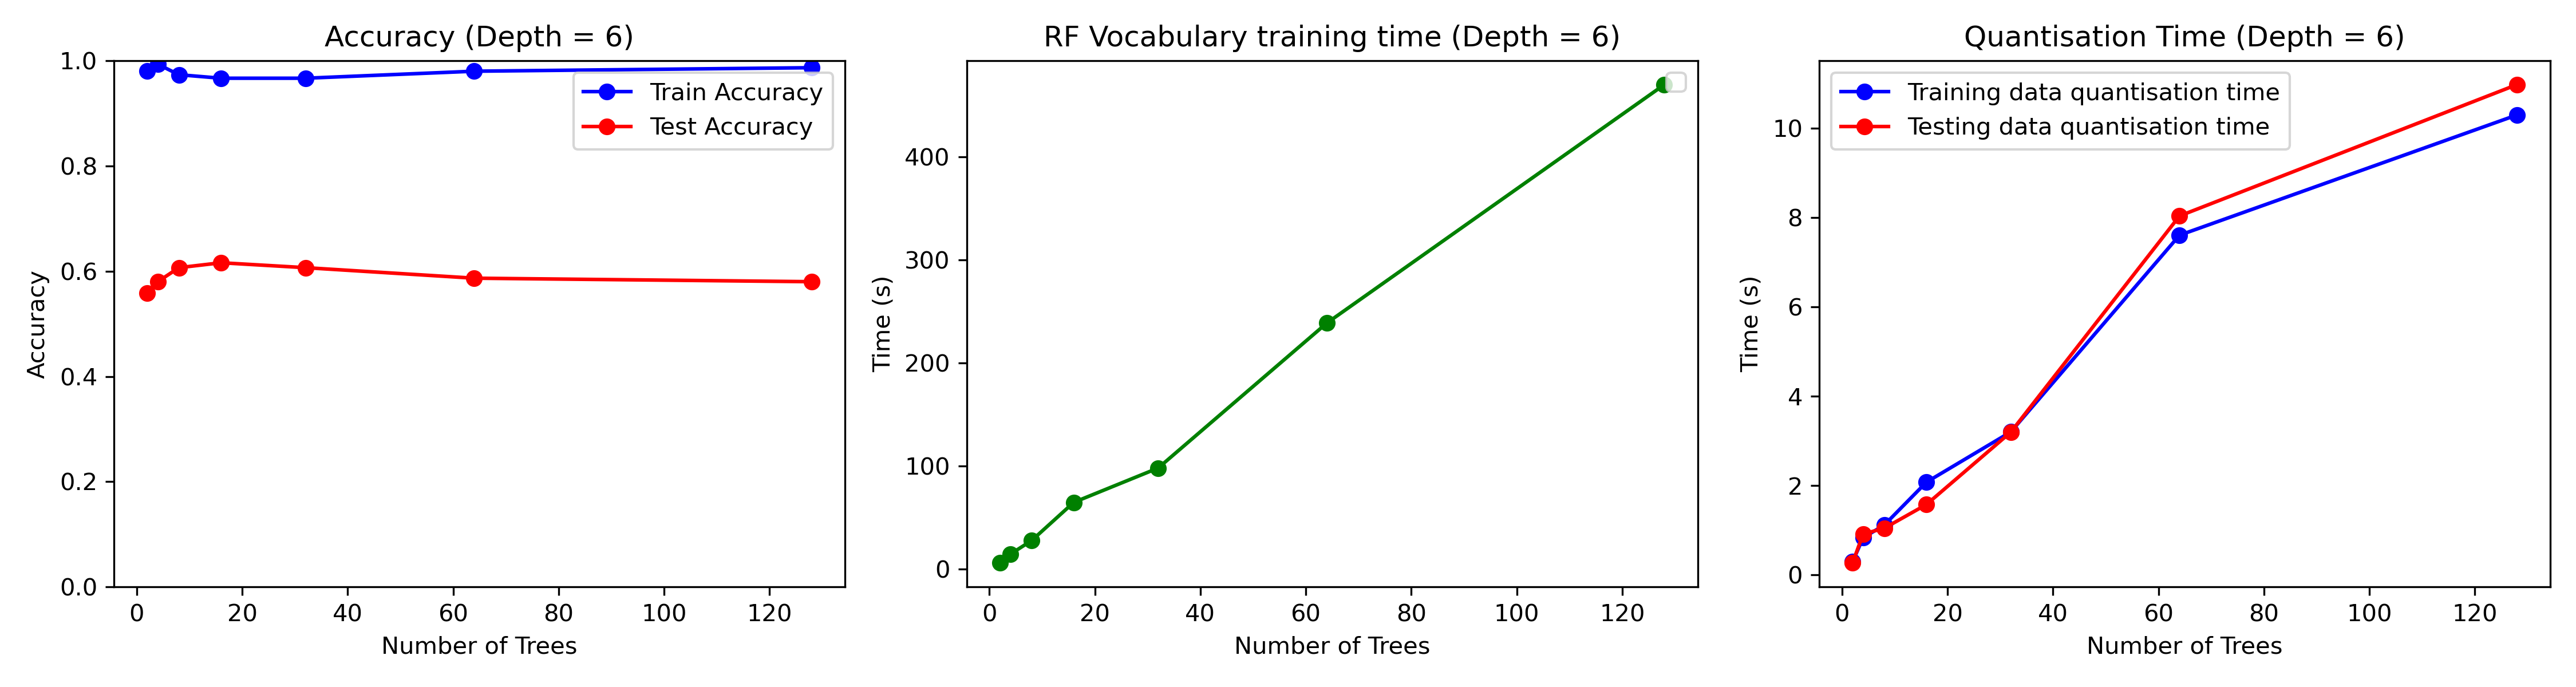
\includegraphics[width=\linewidth]{image/q3-fig2.png}
		\caption{Training\&Testing accuracy and time according to the number of tree (D = 6)}
		\label{fig:q3-fig2}
	\end{subfigure}
	\begin{subfigure}[H]{0.7\linewidth}
		\centering
		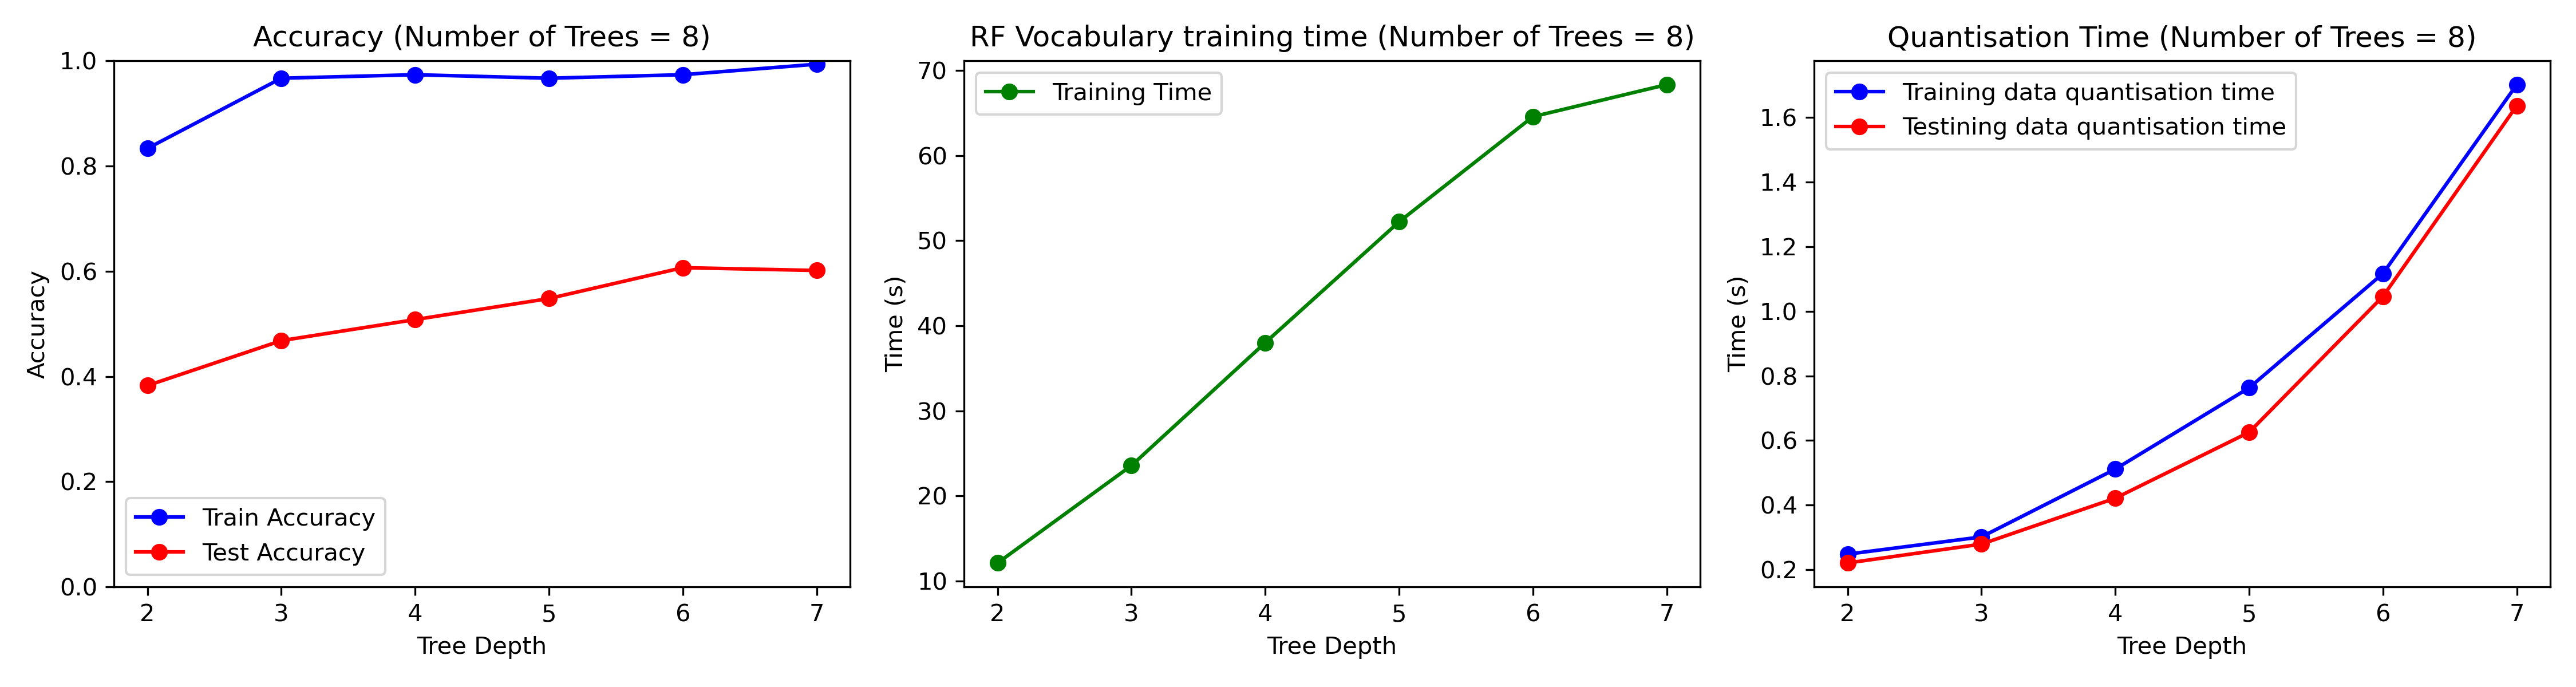
\includegraphics[width=\linewidth]{image/q3-fig3.png}
		\caption{Training\&Testing accuracy and time according to the depth of tree (N = 8)}
		\label{fig:q3-fig3}
	\end{subfigure}
	\caption{Training\&Testing accuracy and time according to the number and depth of trees}
	\label{fig:q3-app-fig1}
\end{figure}


\begin{figure}[htbp]
	\centering
	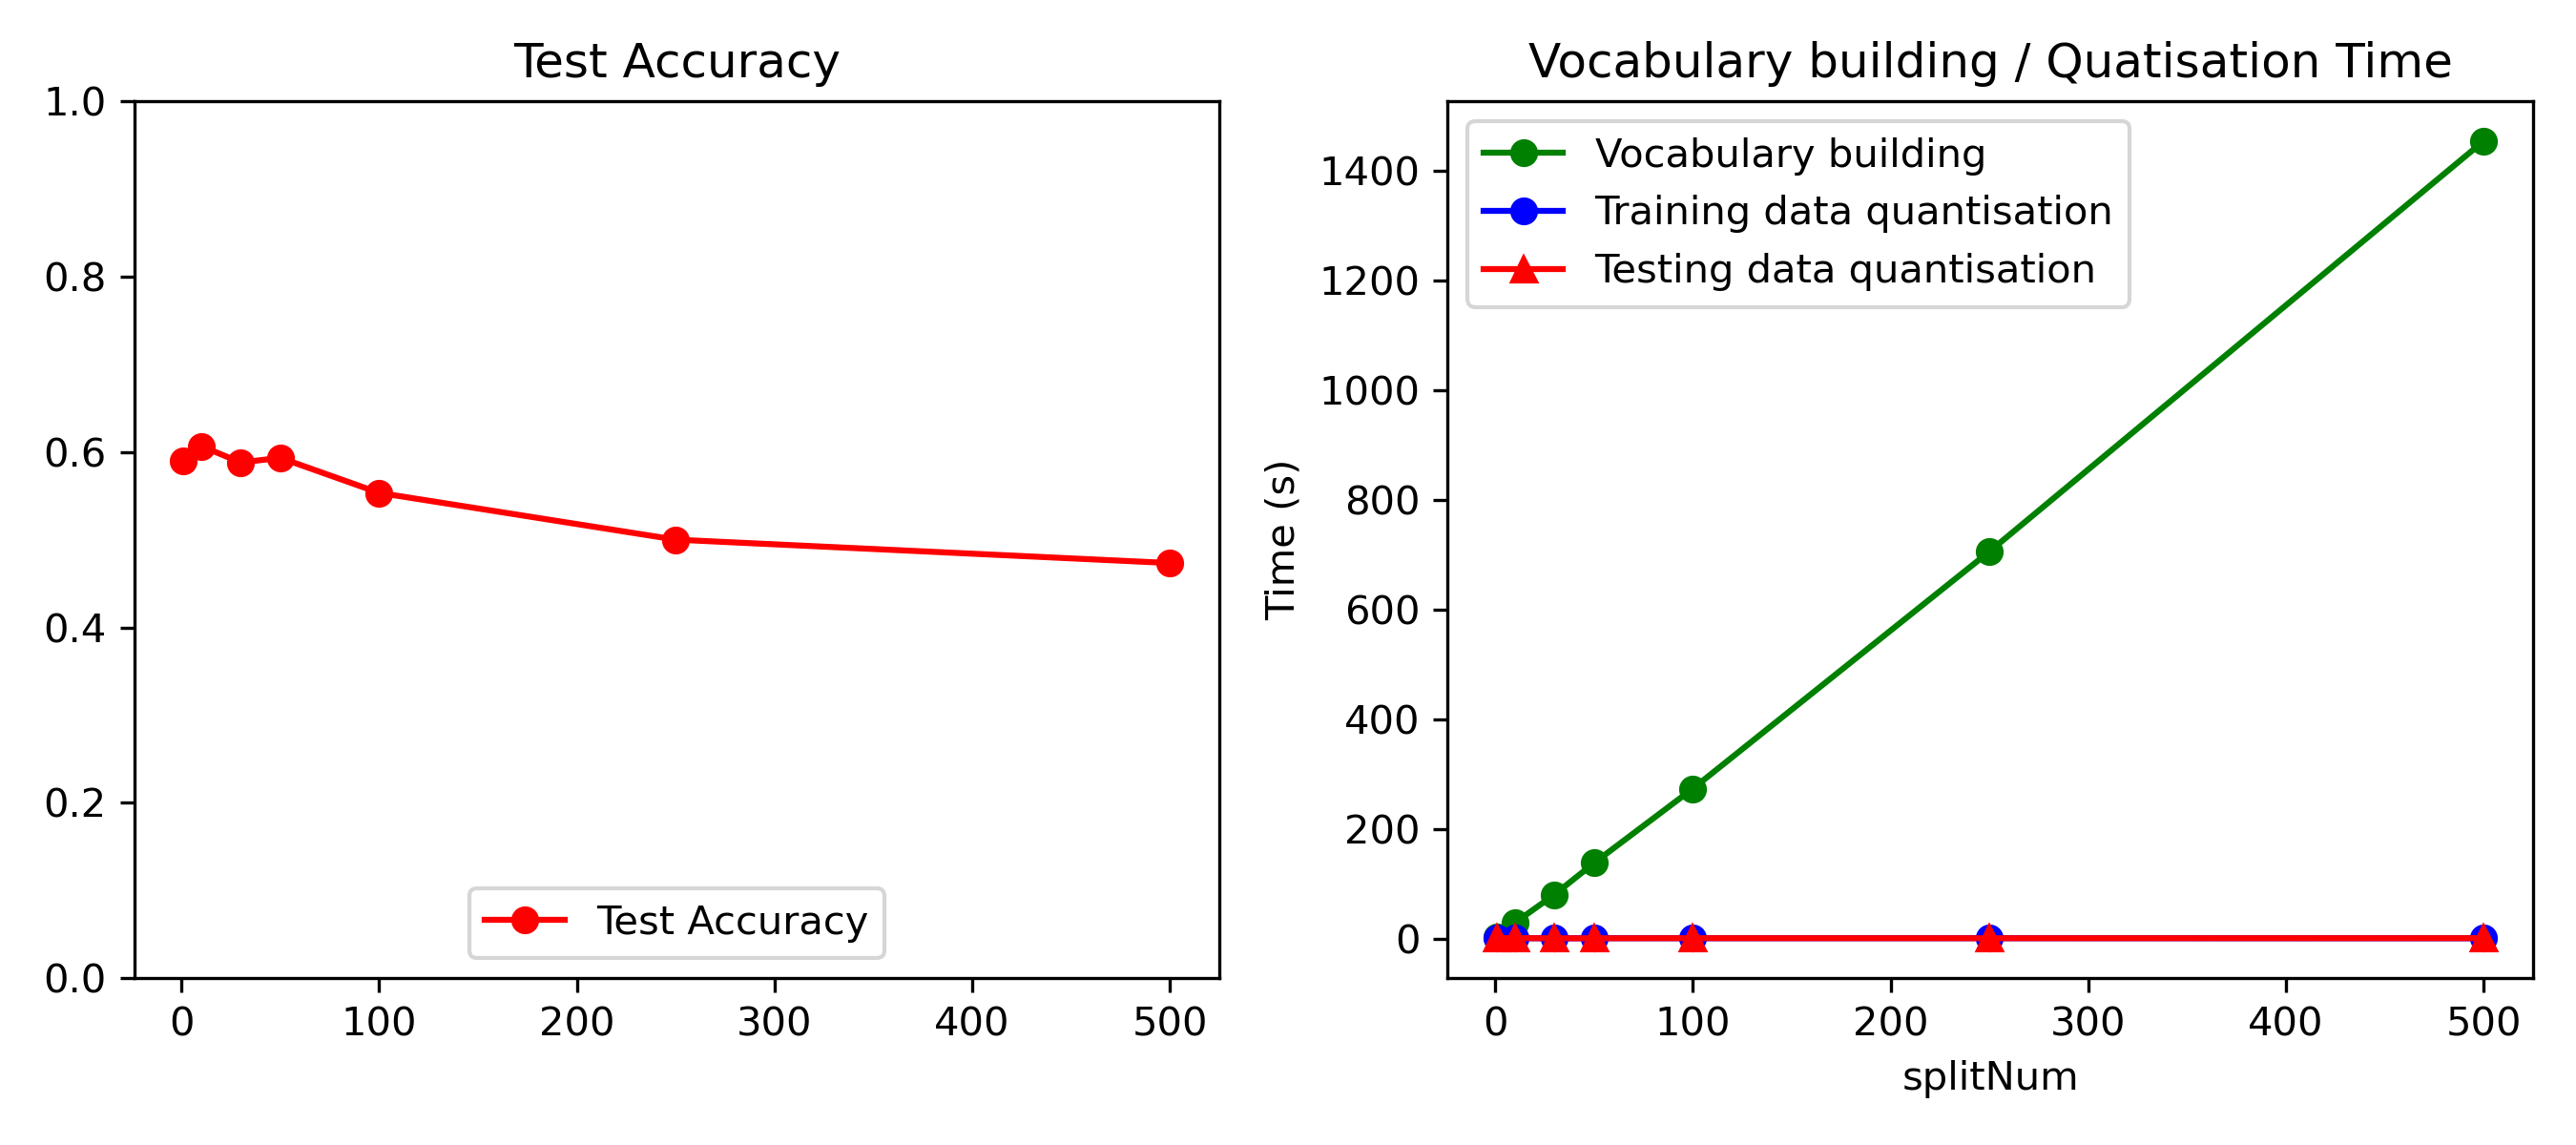
\includegraphics[width=0.5\linewidth]{image/q3-fig5.png}
	\caption{Training\&Testing accuracy and time according to the randomness parameter}
	\label{fig:q3-app-fig2}
\end{figure}

\section{Q3: K-means and Random forest vocabularies' theoretical properties}
\label{subsec:Q3-app1}
To analyze the differences between the k-means vocabulary and the random forest vocabulary, we have examined the theoretical time and space complexities, as shown in \cref{table:q3-app-1}. The definitions of the parameters used are provided below.
\begin{itemize}
	\item $n$: number of training data's feature descriptors (=100K)
	\item $n'$: number of testing data's feature descriptors
	\item $d$: dimension of feature descriptors (=128)
	\item $N$: number of random forest trees
	\item $D$: depth of random forest trees
	\item $K$: k-means vocabulary's size (in random forest, it is same as $2^{D-1} \times N$)
\end{itemize}

Also, although we did not parallelize each tree running of random forest, which took much time compared to k-means vocabulary, theoretically, it has the following advantages. 
\begin{enumerate}
	\item \textbf{Independence from Feature Dimension:} 
	In k-means vocabulary, as the feature dimension increases, the time complexity for both vocabulary building and vector quantization increases linearly due to the need to compute the L2 distance between data points and centroids. In contrast, random Forest maintains constant time complexity with respect to the feature dimension, making it more efficient as the number of features grows. Furthermore, if the feature dimension is extremely large, it can avoid the curse of dimensionality.
	
	\item \textbf{Scalability with Vocabulary Size:} 
	When increasing the vocabulary size, K-means experiences a linear increase in both vocabulary building time and vector quantization time, as both are proportional to the number of clusters. On the other hand, Random Forest scales logarithmically with vocabulary size, as the complexity is divided between the number of trees and the tree depth.
\end{enumerate}

\begin{table}[htbp]
	\centering
	\setlength{\tabcolsep}{6pt} % Adjust column spacing
	\renewcommand{\arraystretch}{1.5} % Adjust row height
	\resizebox{0.5\textwidth}{!}{ % Scale table to fit text width
		\begin{tabular}{|c||c|c|}
			\hline
			& K-means & Random Forest \\ \hline\hline
			Vocabulary building time & $O(Kd n)$ & $O(N D \rho n)$ \\ \hline
			Vector quantisation time & $O(Kd n')$ & $O(N D n')$ \\ \hline
			Space complexity & $O(K d)$ & $O(2^{D} \times N)$ \\ \hline
		\end{tabular}
	}
	\caption{Theoretical properties of vocabulary method: K-means and RF}
	\label{table:q3-app-1}
\end{table}

\section{Q3: Difference between K-means and RF vocabularies' quantisation result}
In \cref{fig:q3_histogram_tr} and \cref{fig:q3_histogram_te}, we compare the quantization results of train and test data using k-means and random forest vocabularies. Each histogram are arranged in the same order as images in \cref{subsec:Q1_histograms}. The random forest results show that the y-labels of the histograms are almost identical and exhibit a relatively uniform distribution. In contrast, the k-means results show significant differences in the y-labels of the histograms depending on the image, producing sparse vectors.

\label{subsec:Q3-app2}
\begin{figure}[htbp]
	\centering
	\begin{subfigure}[t]{0.5\linewidth}
		\centering
		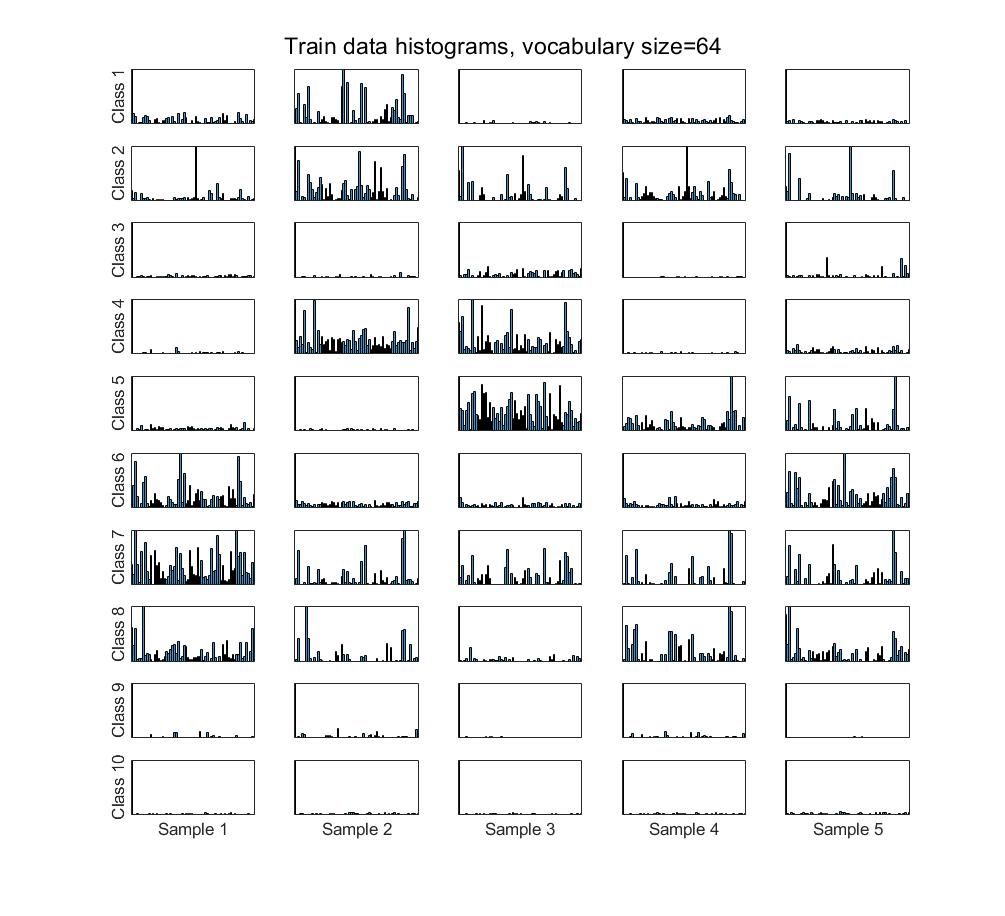
\includegraphics[height=7.5cm]{image/q1-appendix/train_64.png} 
		\caption{K-means vocabulary, $K=64$ (Train data quantisation result)}
	\end{subfigure}%
	\hfill
	\begin{subfigure}[t]{0.5\linewidth}
		\centering
		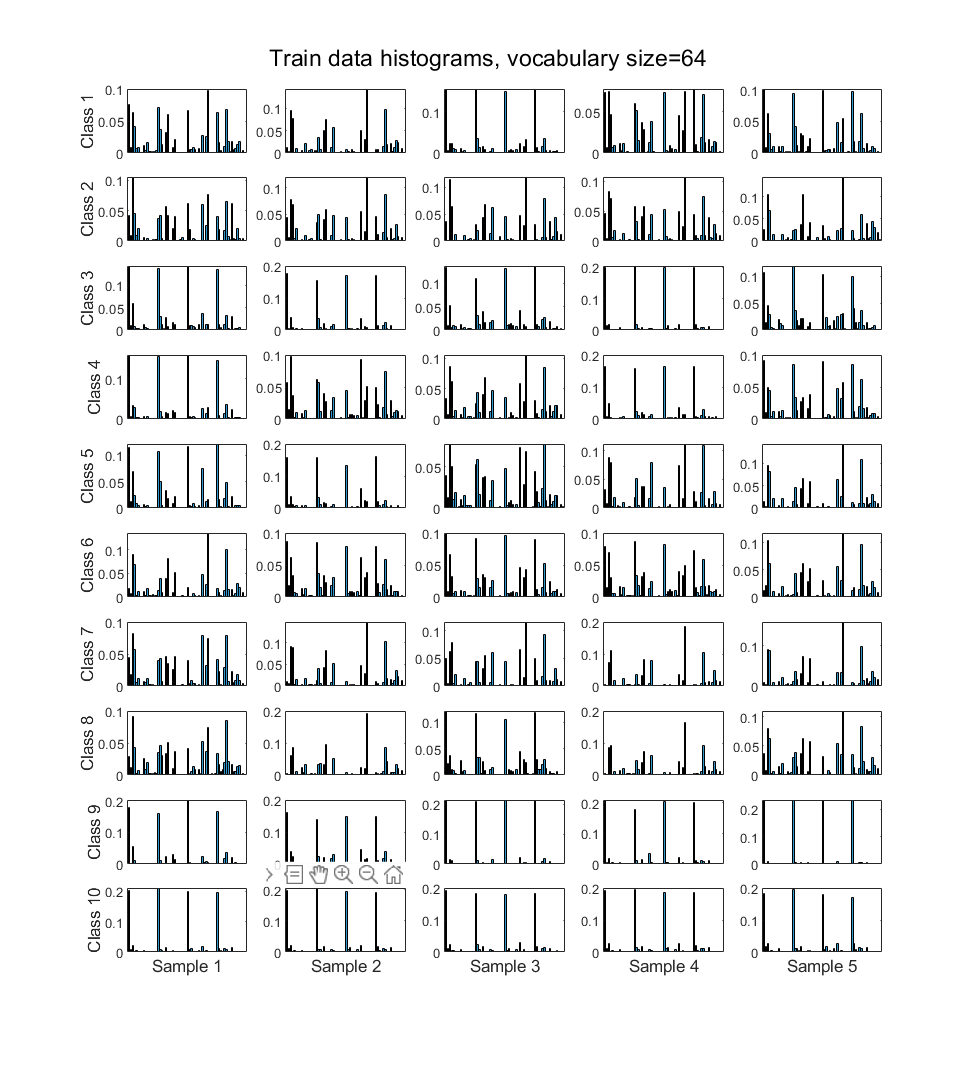
\includegraphics[height=7.5cm]{image/q3-appendix/RFtrain-64.png}
		\caption{Random forest vocabulary, treenum=4 \& treedepth=5 (Train data quantisation result)}
	\end{subfigure}
	
	\centering
	\begin{subfigure}[t]{0.5\linewidth}
		\centering
		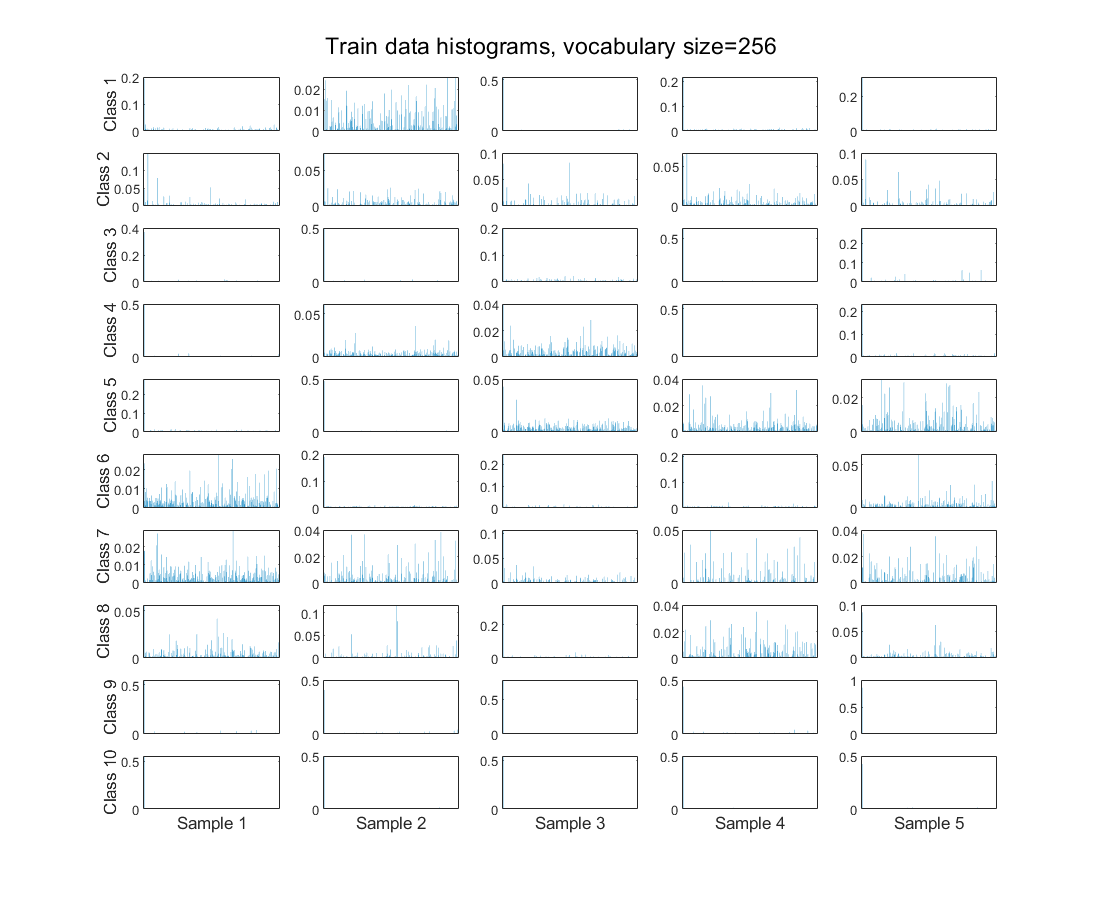
\includegraphics[height=7.5cm]{image/q3-appendix/Kmtrain-256.png} 
		\caption{K-means vocabulary, $K=256$ (Train data quantisation result)}
	\end{subfigure}%
	\hfill
	\begin{subfigure}[t]{0.5\linewidth}
		\centering
		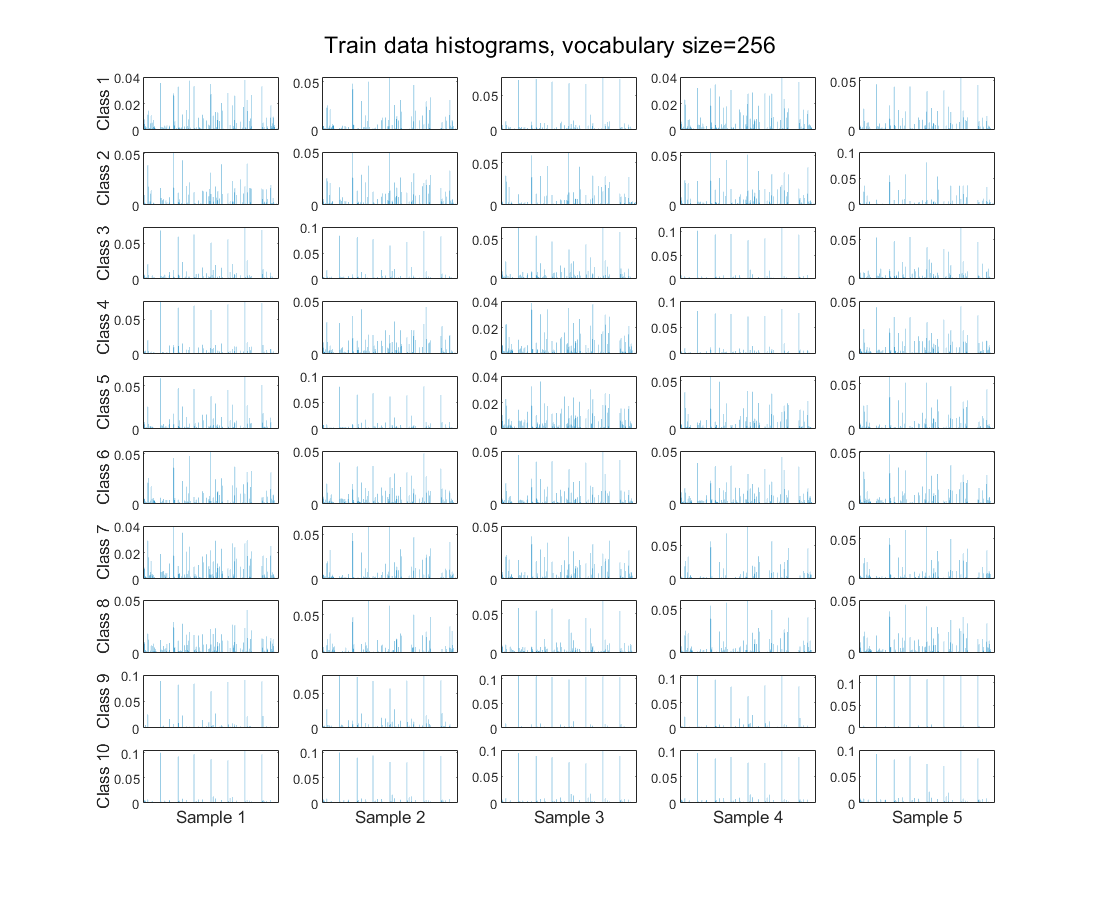
\includegraphics[height=7.5cm]{image/q3-appendix/RFtrain-256.png}
		\caption{Random forest vocabulary, treenum=8 \& treedepth=6 (Train data quantisation result)}
	\end{subfigure}

	\caption{K-means vs Random forest vocabulary: Visualistaion of train data quantisation result}
	\label{fig:q3_histogram_tr}
\end{figure}

\begin{figure}[htbp]
	\centering
	\begin{subfigure}[t]{0.5\linewidth}
		\centering
		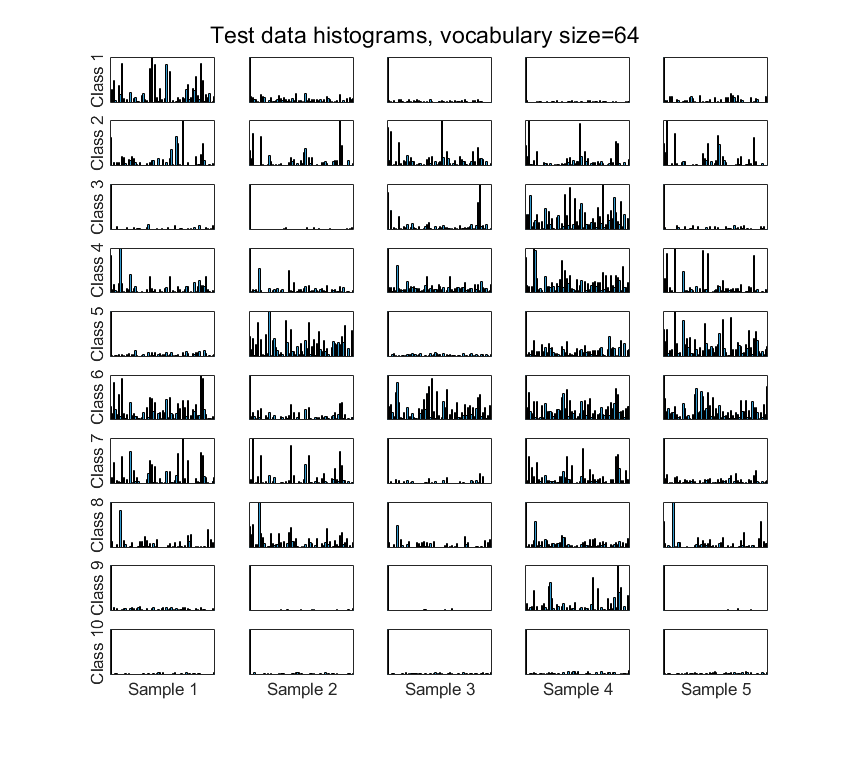
\includegraphics[height=7.5cm]{image/q1-appendix/test_64.png} 
		\caption{K-means vocabulary, $K=64$ (Testn data quantisation result)}
	\end{subfigure}%
	\hfill
	\begin{subfigure}[t]{0.5\linewidth}
		\centering
		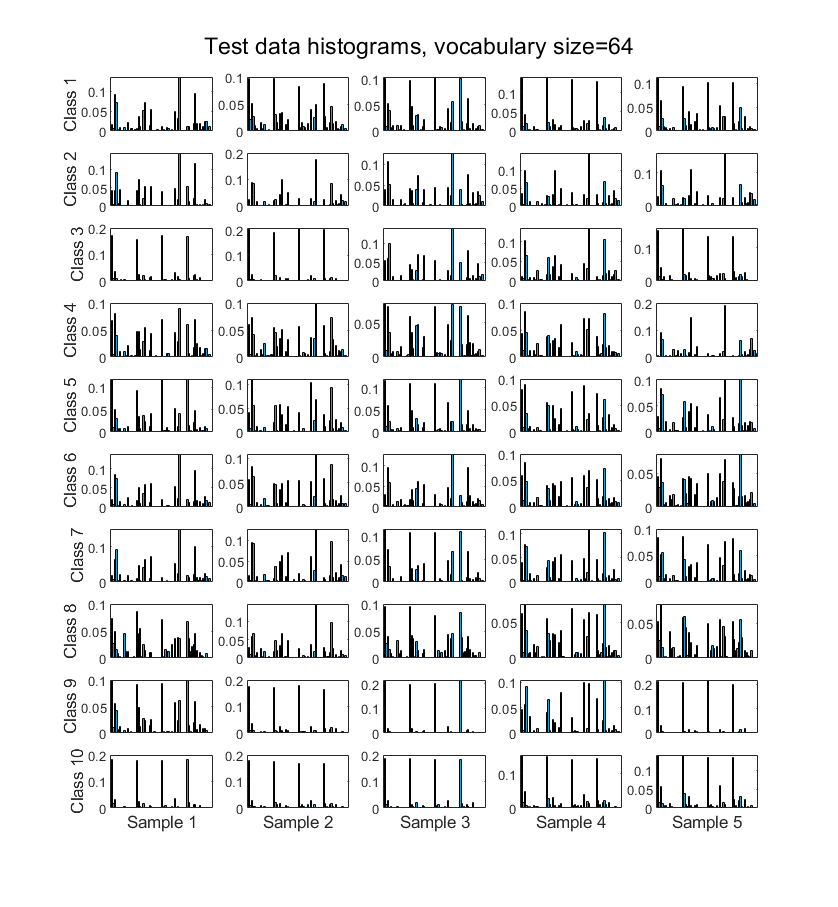
\includegraphics[height=7.5cm]{image/q3-appendix/RFtest-64.png}
		\caption{Random forest vocabulary, treenum=4 \& treedepth=5 (Test data quantisation result)}
	\end{subfigure}
	
	\centering
	\begin{subfigure}[t]{0.5\linewidth}
		\centering
		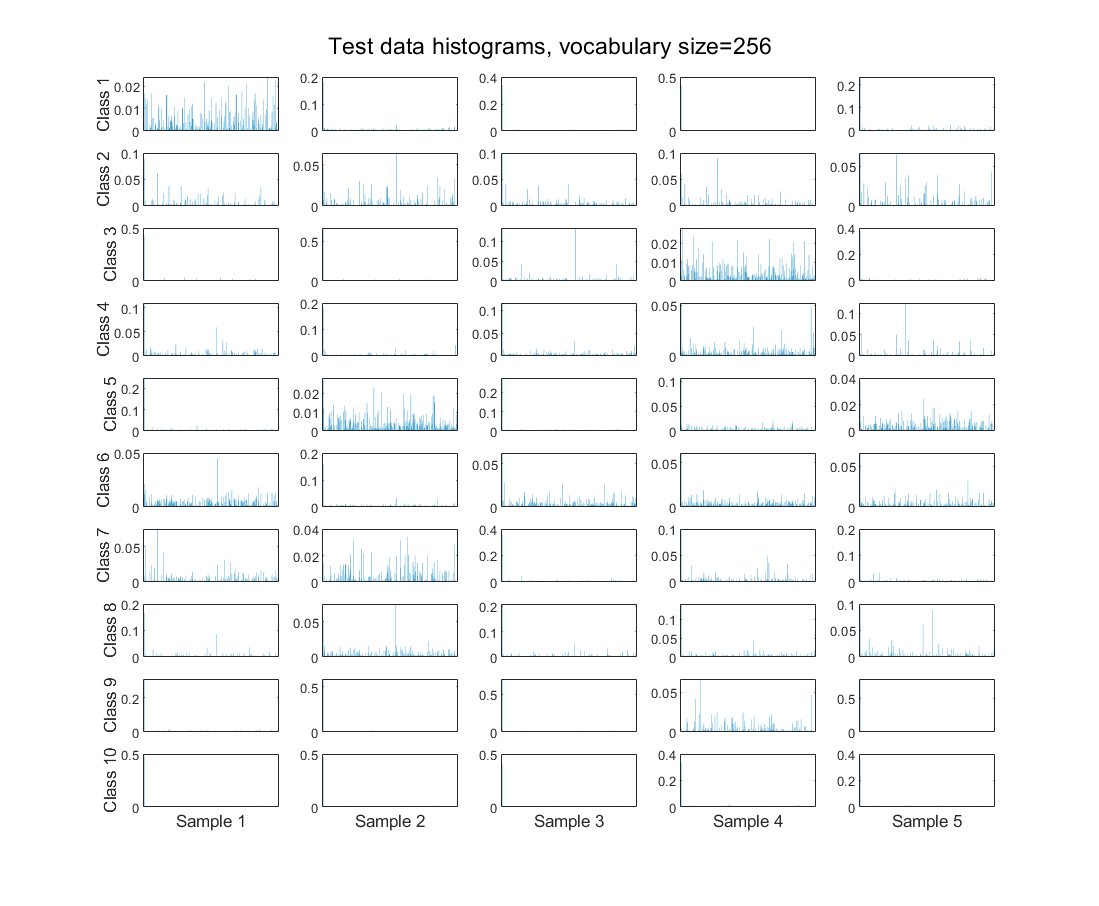
\includegraphics[height=7.5cm]{image/q3-appendix/Kmtest-256.png} 
		\caption{K-means vocabulary, $K=256$ (Test data quantisation result)}
	\end{subfigure}%
	\hfill
	\begin{subfigure}[t]{0.5\linewidth}
		\centering
		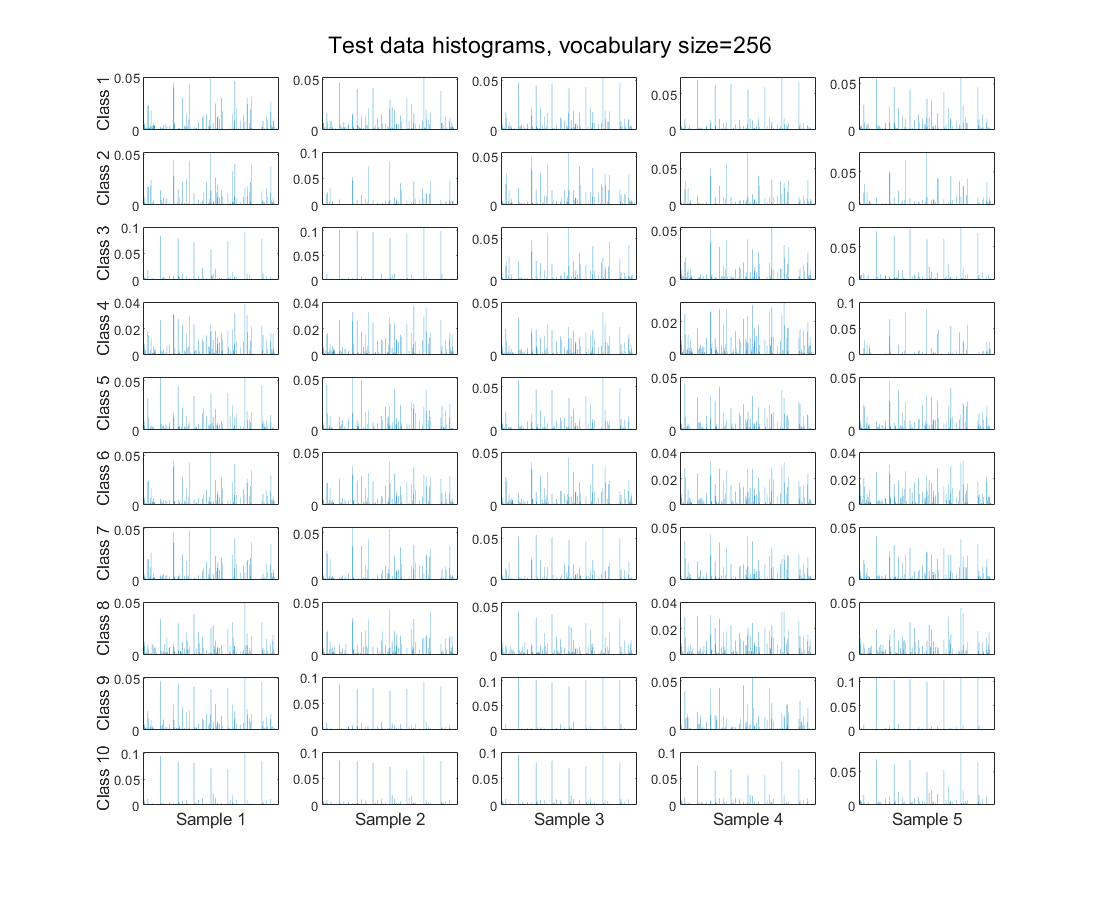
\includegraphics[height=7.5cm]{image/q3-appendix/RFtest-256.png}
		\caption{Random forest vocabulary, treenum=8 \& treedepth=6 (Test data quantisation result)}
	\end{subfigure}
	
	\caption{K-means vs Random forest vocabulary: Visualistaion of test data quantisation result}
	\label{fig:q3_histogram_te}
\end{figure}

\section{Q3: Test result's confusion matrix and success/failure cases}
\label{subsec:Q3-app4}
The optimal parameters determined for the random forest vocabulary through experiments are $N=8$, $D=6$, and $\text{splitnum}=10$. With this configuration, each real-time executable weak learner—axis-aligned and two-pixel tests—each was trained 10 times. The confusion matrix results in \cref{fig:APP-q3-conf} represent the best test accuracy among the 10 repetitive train results.\\
As a result, we can observe that the information gain of the two-pixel test is significantly higher. Referring to \cref{fig:APP-q3-conf}, it is evident that the accuracy for all classes is generally higher in the two-pixel weak learner compared to the axis-aligned weak learner. However, since the random forest vocabulary tends to have higher between-class similarity compared to the k-means vocabulary, it struggles to distinguish images of different classes that share similar features. An example of this is shown in \cref{fig:APP-q3-case2} and \cref{fig:APP-q3-case4}, where the circular feature of the watch is mistakenly classified as similar to the curved shapes of objects like the wheelchair and Windsor chair.\\
You can see the example success and failure cases of random forest codebook at \cref{fig:APP-q3-case1}, \cref{fig:APP-q3-case2}, \cref{fig:APP-q3-case3} and \cref{fig:APP-q3-case4}.

\begin{figure}[htbp]
	\centering
	\begin{subfigure}[t]{0.4\linewidth}
		\centering
		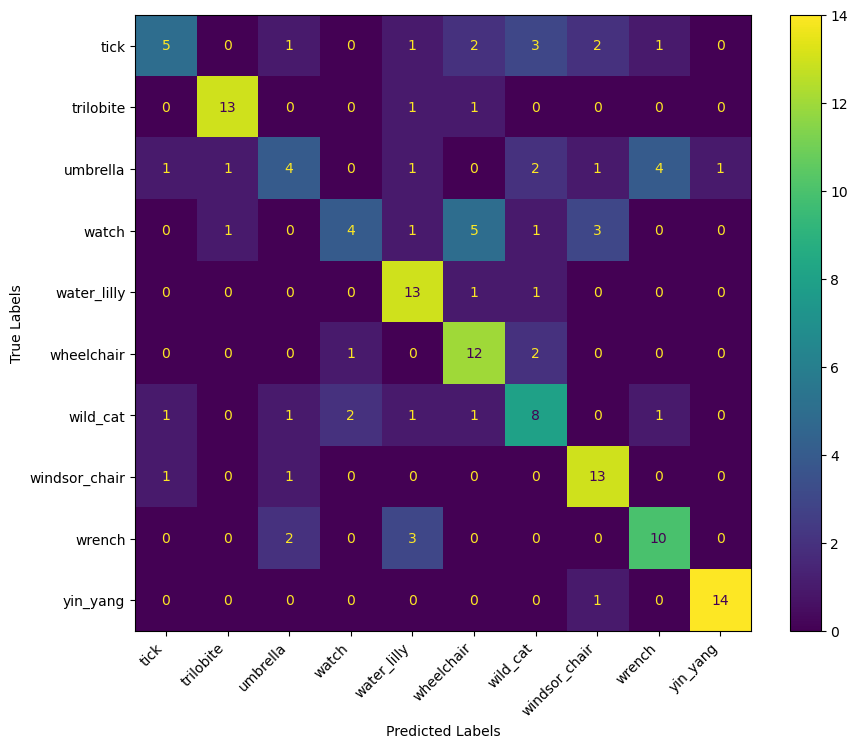
\includegraphics[width=\linewidth]{image/conf-appendix/rf_axis_confusion.png}
		\caption{Axis-aligned weak learner, test accuracy=0.640}
		\label{fig:q3-appfig1}
	\end{subfigure}%
	\quad
	\begin{subfigure}[t]{0.4\linewidth}
		\centering
		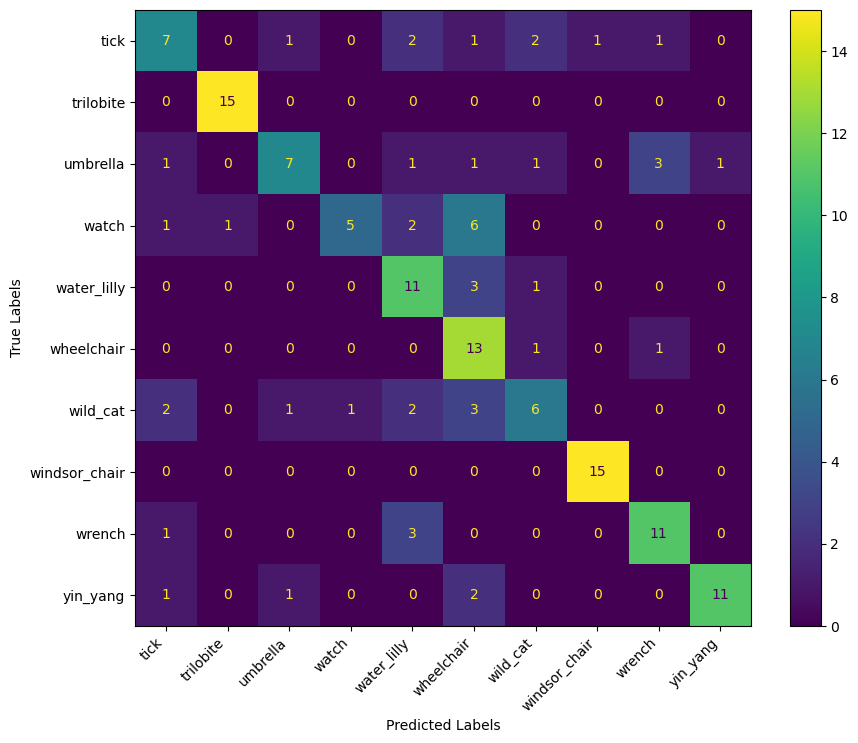
\includegraphics[width=\linewidth]{image/conf-appendix/rf_two_confusion.png}
		\caption{Two-pixel test weak learner, test accuracy=0.673}
		\label{fig:q3-appfig2}
	\end{subfigure}
	\caption{Confusion matrix of optimal cases ($N=250$, $D=8$, and $\text{splitnum}=10$) with K-means codebook}
	\label{fig:APP-q3-conf}
\end{figure}

\begin{figure}[htbp]
	\centering
	\begin{subfigure}{0.45\linewidth}
		\centering
		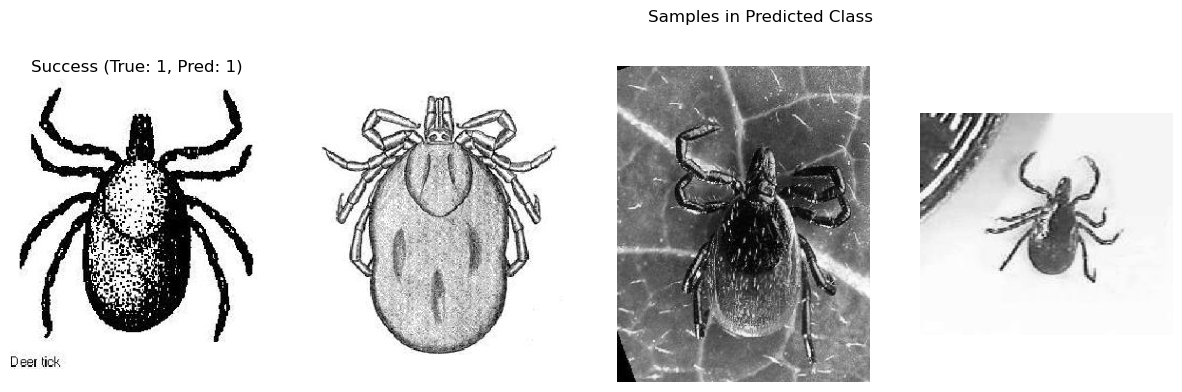
\includegraphics[width=\linewidth]{image/conf-appendix/rf_axis_succ1.png}
	\end{subfigure}%
	\quad
	\begin{subfigure}{0.45\linewidth}
		\centering
		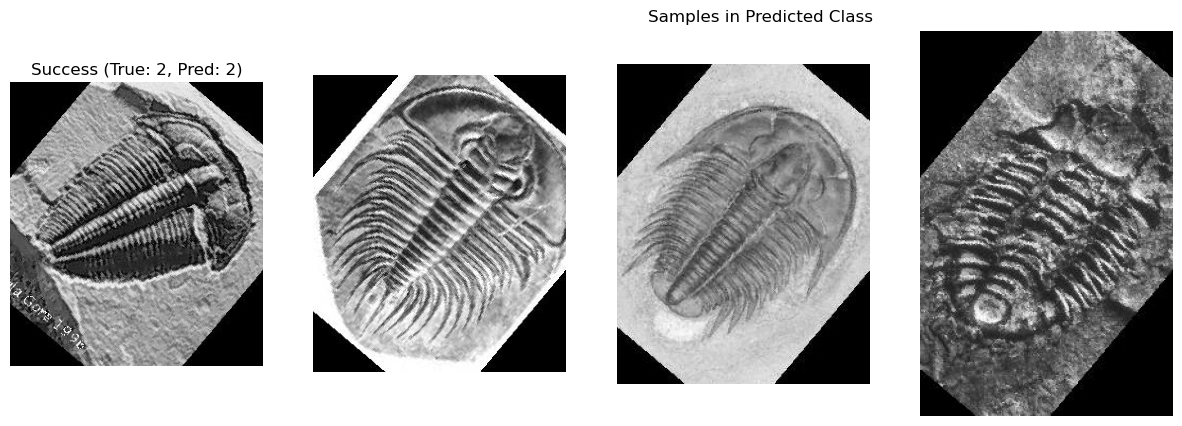
\includegraphics[width=\linewidth]{image/conf-appendix/rf_axis_succ2.png}
	\end{subfigure}
	\caption{RF codebook with axis-aligned weak learner: Example success case}
	\label{fig:APP-q3-case1}
\end{figure}
\begin{figure}[htbp]
	\centering
	\begin{subfigure}[t]{0.45\linewidth}
		\centering
		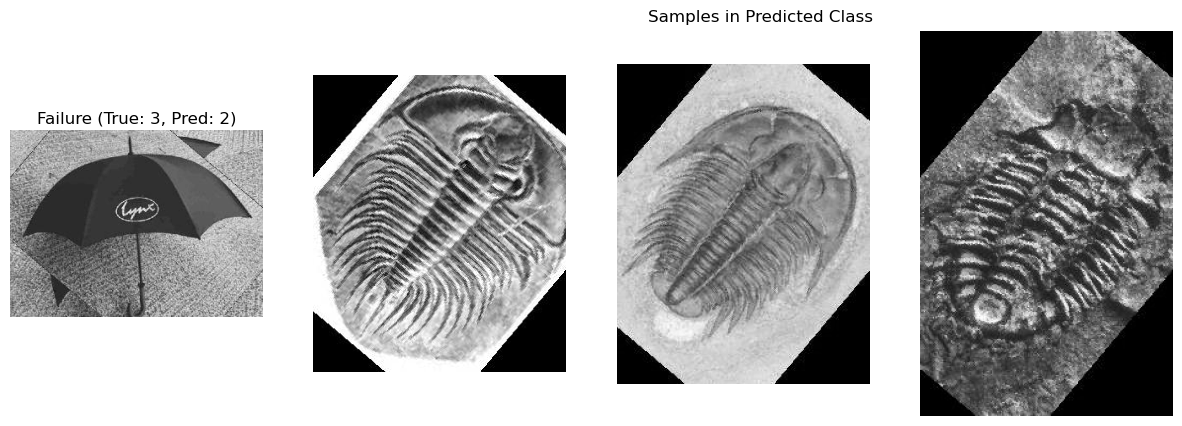
\includegraphics[width=\linewidth]{image/conf-appendix/rf_axis_fail2.png}
	\end{subfigure}%
	\quad
	\begin{subfigure}[t]{0.45\linewidth}
		\centering
		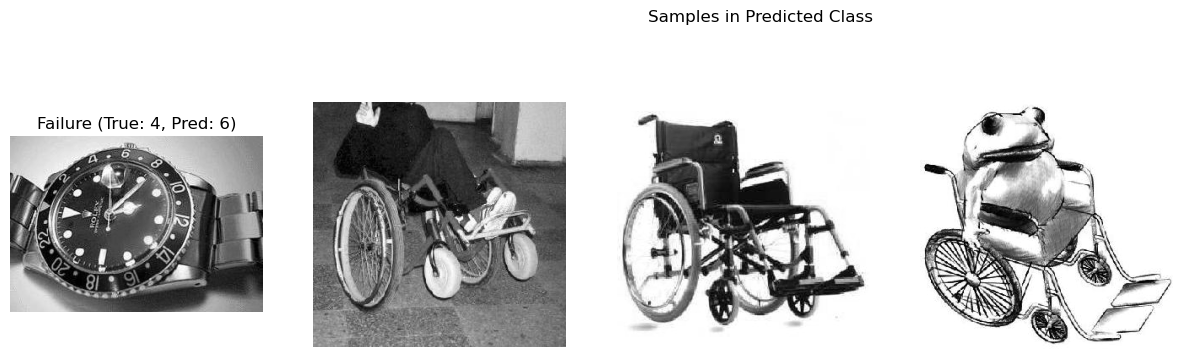
\includegraphics[width=\linewidth]{image/conf-appendix/rf_axis_fail3.png}
	\end{subfigure}
	\caption{RF codebook with axis-aligned weak learner: Example failure case}
	\label{fig:APP-q3-case2}
\end{figure}

\begin{figure}[htbp]
	\centering
	\begin{subfigure}{0.45\linewidth}
		\centering
		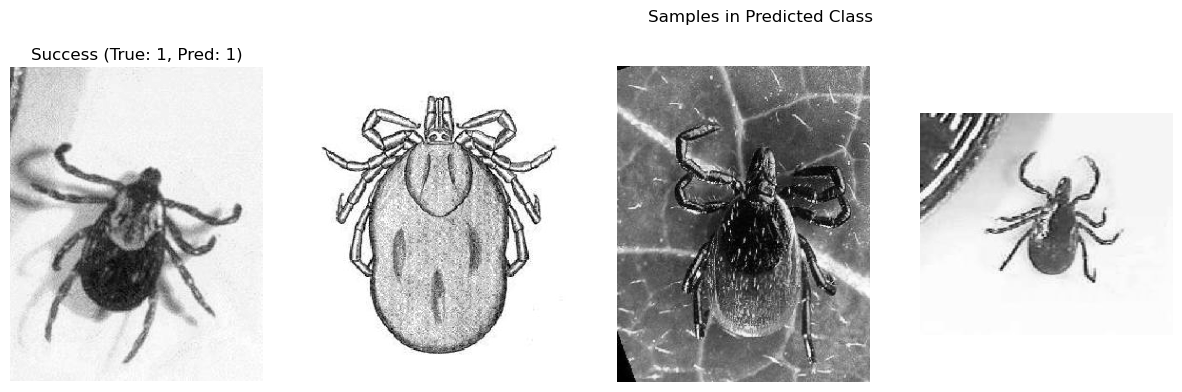
\includegraphics[width=\linewidth]{image/conf-appendix/rf_two_succ1.png}
	\end{subfigure}%
	\quad
	\begin{subfigure}{0.45\linewidth}
		\centering
		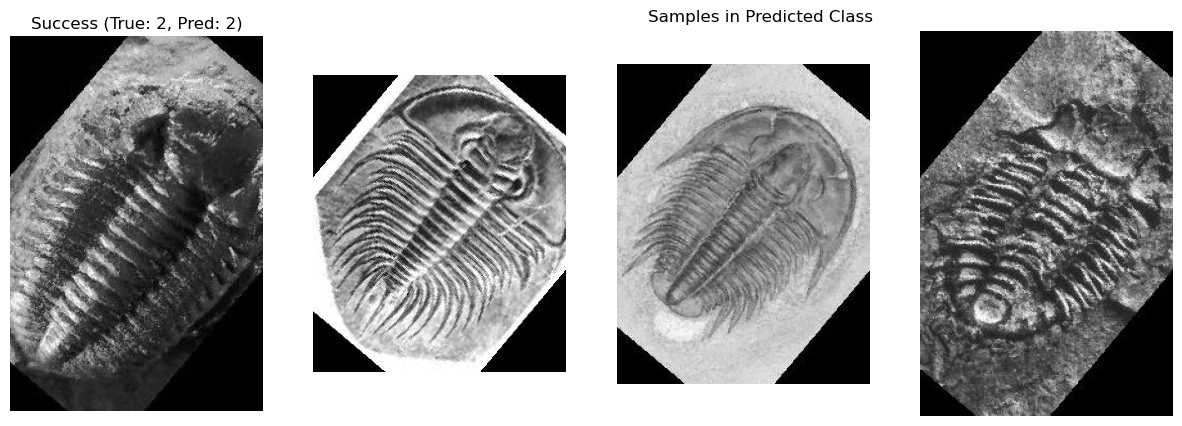
\includegraphics[width=\linewidth]{image/conf-appendix/rf_two_succ2.png}
	\end{subfigure}
	\caption{RF codebook with two-pixel weak learner: Example success case}
	\label{fig:APP-q3-case3}
\end{figure}
\begin{figure}[htbp]
	\centering
	\begin{subfigure}[t]{0.45\linewidth}
		\centering
		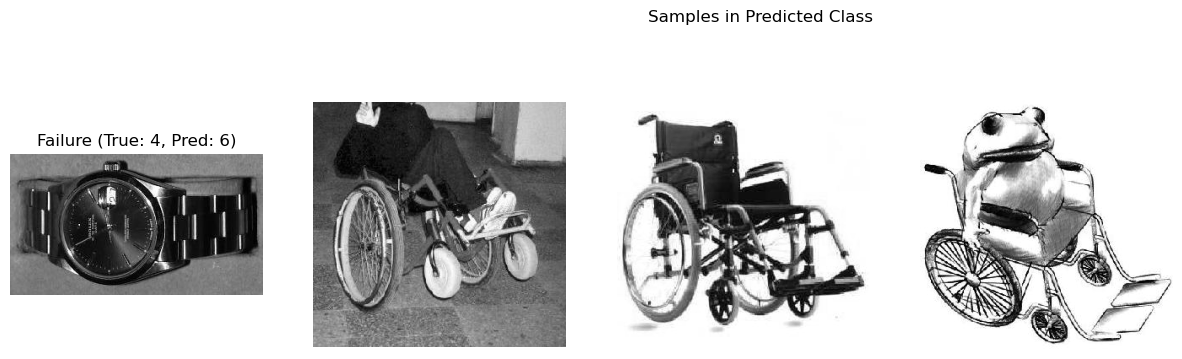
\includegraphics[width=\linewidth]{image/conf-appendix/rf_two_fail1.png}
	\end{subfigure}%
	\quad
	\begin{subfigure}[t]{0.45\linewidth}
		\centering
		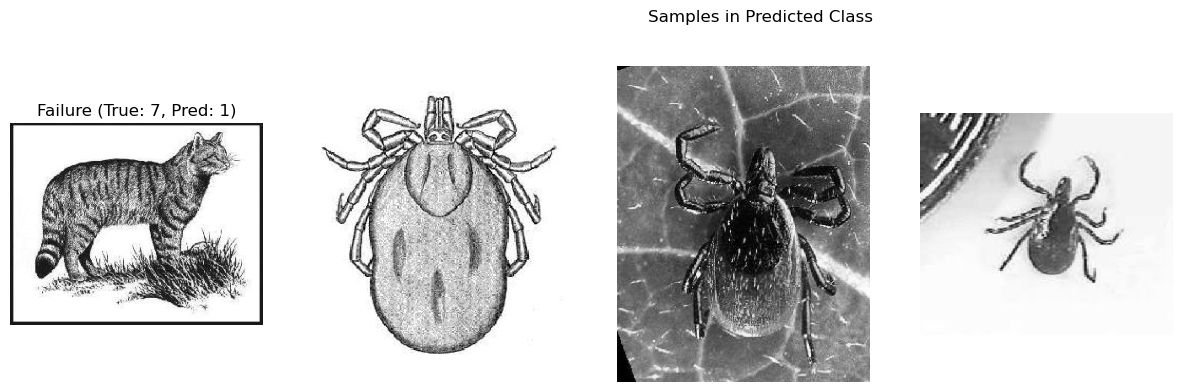
\includegraphics[width=\linewidth]{image/conf-appendix/rf_two_fail2.png}
	\end{subfigure}
	\caption{RF codebook with two-pixel weak learner: Example failure case}
	\label{fig:APP-q3-case4}
\end{figure}